\subsubsection{Jupyter}
\label{sec:jupyter}
\TOWRITE{NT}{Where to put this? It contains a description mostly taken  from the WP5 Userinterfaces description that is now moved here and referred to back here. We need to say early on what Jupyter is, and can then refer back to it in the WorkPackages. We just need to put this in the right place in the concept/approach section...}.
\begin{wrapfigure}{r}{0.50\textwidth}
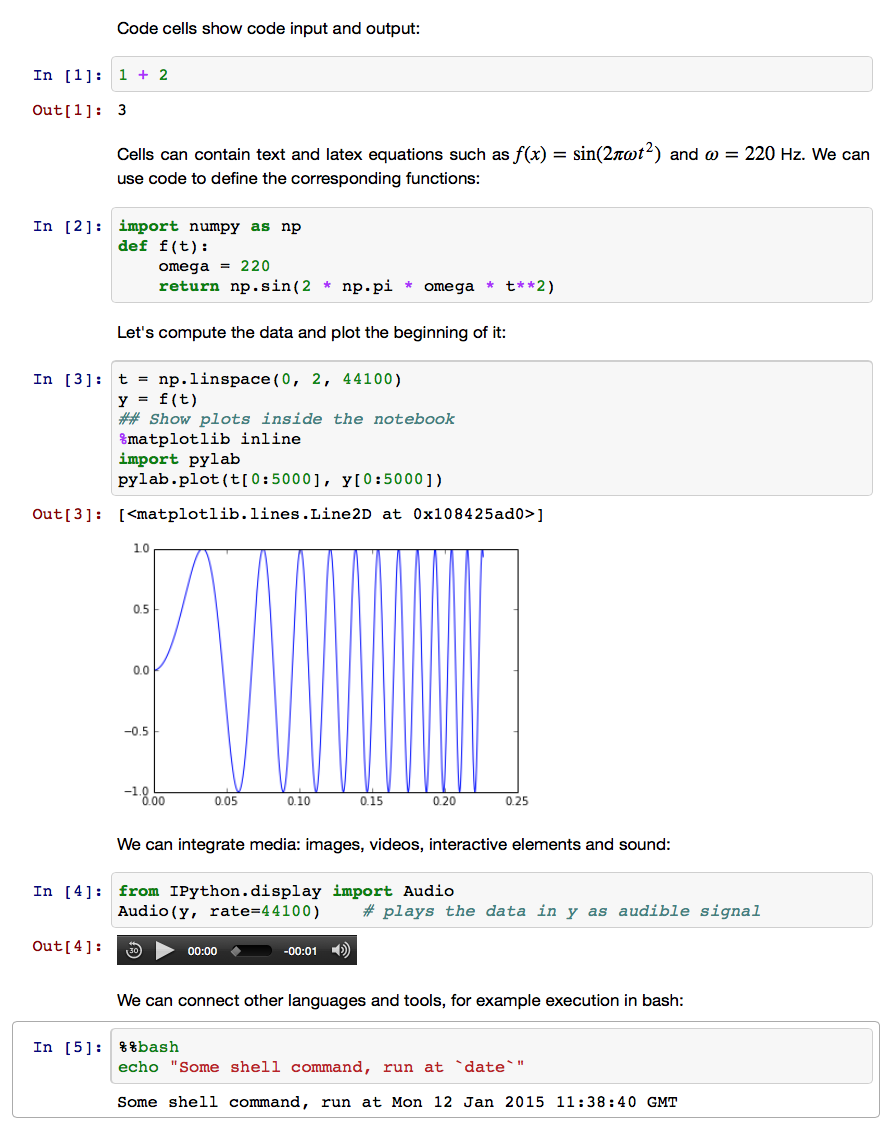
\includegraphics[scale=0.23]{Pictures/jupyterdemo1.png}
\caption{\label{fig:jupyterdemo} A tiny self-contained Notebook demonstrating the concepts of cells that contain different types of material and can be executed (or updated) in arbitrary or sequential order.}
\end{wrapfigure}

Project \Jupyter is a set of open-source software projects for
interactive and exploratory computing. These software projects help
make scientific computing and data science reproducible and
multi-language (Python, Julia, R, Haskell, Bash, R, \ldots). The main
application offered by \Jupyter is the \Jupyter notebook, a unique
web-based interactive computing platform that allows users to create
data- and code-driven narratives that combine live (re-executable)
code, equations, narrative text, interactive dashboards and other rich
media. 

Figure~\ref{fig:jupyterdemo} shows a Python-based sample
session. Within the Python session, all libraries available in Python
can be imported and combined flexibly, a number of interfaces between
different languages exist. Many more examples are available, for
example \cite{IPython-demo-hyperbolic-conservation-laws} and
within \cite{IPython-sload-foundation-report-2013}.

The \Jupyter notebook is being used in all areas of academic
(including for example University of California, Berkeley, Stanford,
MIT, Harvard, Cambridge, Oxford, Imperial College, Southampton,
Hamburg, Paderborn, Vienna, Paris, Katowice, and Oslo) and government
(NASA JPL, LBL, KBase, White House Hackathon) research as well as
industry (Google, IBM, Facebook, Oracle, Otto Group, Microsoft,
Bloomberg, JP Morgan, WhatsApp, O’Reilly, Quantopian, Logilab,
GraphLab, Enthought, Continuum, Authorea, BuzzFeed, etc.)  and
journalism (538, New York Times, etc.). \\
%
Because the architecture and building blocks of \Jupyter are open,
they are being used to build numerous other commercial and non-profit
products and services. The \Jupyter Notebook has between 500,000 and
1.5 million individual users worldwide.

These notebook documents provide a complete and executable record of a
computation that can be shared with others in a way that has not been
possible before. This has led, among other things, to a huge boost in
reproducible, interactive teaching/education documents in recent
years.

We will build on this technology by extending \Jupyter with new
functionality, unifying other computational tools to be usable as
components in this framework, and merging the \Sage and \Jupyter
development.
\TOWRITE{NT}{Is the 'merge' too strong a claim? Please correct / remove.}



